% !TEX root = SocialVision2012.tex

\subsubsection{Detecting and recognizing proxemes}
\label{subsec:activity}
\vspace{-5pt}
A key benefit of the proposed representations is that they enable efficient and robust comparisons between interactions, allowing applications from recognition to clustering (i.e., unsupervised learning of proxemes). To demonstrate this, preliminary results of detecting and recognizing pre-defined social proxemes from videos using this simple representation are presented in \cite{groupdet2013} by the PIs.

%We approach detection and recognition as a matching problem, depicted in the left of Fig.~\ref{fig:diagram_dataset}. Suppose we have an exemplar from an interaction category involving $N$ participants, and we wish to localize within a long video of a larger social gathering ($M>N$ tracks) the times and locations in which sub-groups of agents participate in similar interactions. To succeed, we must deal with some of the $M$ tracks being artifacts caused by false detections, and others being fragmented due to tracking breakdowns and agent exits. We must also account for interactions occurring over different temporal extents and at variable rates within their extents.

In this system, detecting and recognizing pre-defined social proxemes is posed as a matching problem, depicted in the left of Fig.~\ref{fig:diagram_dataset}. Suppose we have an exemplar of a proxeme involving $N$ participants, and we wish to localize within a long video of a larger social gathering ($M>N$ tracks) the times and locations in which sub-groups of agents participate in similar interactions. To succeed, we must deal with some of the $M$ tracks being artifacts caused by false detections, and others being fragmented due to tracking breakdowns and agent exits. We must also account for interactions occurring over different temporal extents and at variable rates within their extents.

\begin{figure}[t!]
\begin{center}
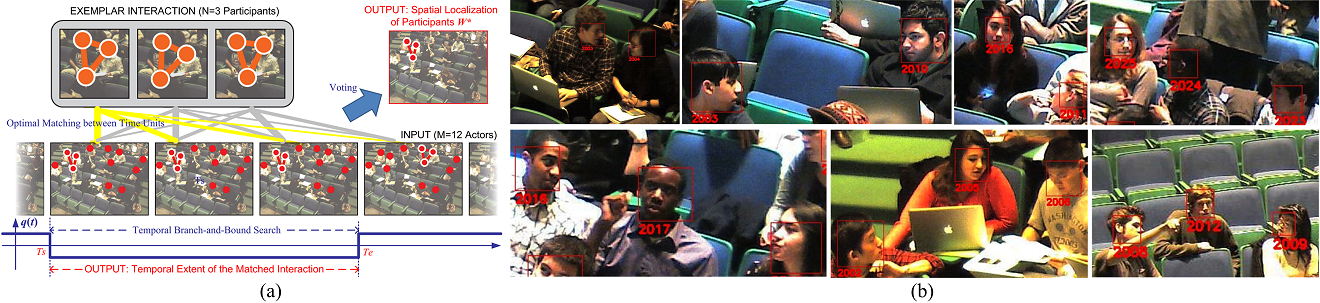
\includegraphics[width=\columnwidth]{groupdet2013}
\end{center}
\vspace{-0.25in} \caption{\captionsize 
(a): Preliminary system for detecting and recognizing social proxemes using the proposed representation. (b): Examples of the educationally-meaningful proxemes.}
\label{fig:diagram_dataset}\afterfigspace
\end{figure}


To deal with these various sources of noise and outliers, each frame of the exemplar is separately compared to each frame of the long input video, and for each comparison we find the optimal partial matching between the $N$ exemplar participants and the $M>N$ input tracks. Each frame-wise partial match is represented by an $N\times M$ binary matrix $W$ that has at most one non-zero entry in each row and column. Because our descriptor-ensembles include only unitary and pairwise descriptors, each partial match can be found efficiently using a quadratic program similar to that used in shape matching \cite{Berg05shapematching}
\begin{equation}\label{eq:partial-matching}
\text{arg}\!\!\!\!\!\min_{W=\{w_{nm}\}} \sum_{nm}w_{nm}d_{I}(\mathbf{f}_{m}, \mathbf{f}_{n})+\!\!\!\sum_{nmn'm'}\!\!\!w_{nm}w_{n'm'}d_{P}(\mathbf{g}_{m,m'}, \mathbf{g}_{n,n'}),
\end{equation}
where $\{\mathbf{f}_{n},\mathbf{g}_{n,n'}\}$ is the collection of $N$ individual and $N\times (N-1)$ pairwise descriptors from one exemplar frame and $\{\mathbf{f}_{m},\mathbf{g}_{m,m'}\}$ are the $M$ and $M\times (M-1)$ individual and pairwise descriptors from one frame of the input. We can explore many different ``atomic'' distances for comparing individual and pairwise descriptors, and so far we have experimented with one flexible and convenient choice based on Mahalanobis distance: $d_{I}(\mathbf{f}, \mathbf{f}')=(\mathbf{f}-\mathbf{f}')^{T}\Sigma_{I}(\mathbf{f}-\mathbf{f}')$ and $d_{P}(\mathbf{g}, \mathbf{g}')=(\mathbf{g}-\mathbf{g}')^{T}\Sigma_{P}(\mathbf{g}-\mathbf{g}')$ defined by data-optimized positive semi-definite matrices $\Sigma_{I}$ and $\Sigma_{P}$. Having computed all per-frame partial matches, we make a robust decision about the locations of the $N$ best-matching participants in the input video by accumulating weighted votes from these frame-wise matches, with each frame-wise match casting a vote in the discrete space of all possible $N\times M$ binary matching matrices. Once the best-matching $N$ participants have been identified, we have found that the temporal extent of the interaction can be found efficiently through a suitably-defined branch-and-bound temporal search\comment{ inspired by techniques used in object detection~\cite{Lampert}}. As discussed in \cite{groupdet2013}, this computational mechanism is robust to false detections and insensitive to moderately broken tracks.


%\todd{Working here}. To formally describe task consider the fact that if one of the $M$ targets is regarded as a participant in an interaction as exemplified by the exemplar $\mathcal{D}$, its behavior should properly match to the behavior of one of the $N$ individuals in the exemplar $\mathcal{D}$. Therefore, we use a $N\times M$ binary matrix $W=[w_{nm}]\in\{0,1\}^{N\times M}$ to formally represent the participant identification, where $w_{nm}=1$ means that the $n$th exemplar individual is matched to the $m$th input target and $w_{nm}=0$ means unmatched targets. For unambiguous matching, we expect each individual in the exemplar to find its unique partner target in the input. This implies that $\sum_{m}w_{nm}=1, \forall n$ and $\sum_{n}w_{nm}\leq 1, \forall m$, \textit{i.e.}, $W\mathbf{1}=\mathbf{1}$ and $\mathbf{1}^{T}W\leq\mathbf{1}^{T}$. Denote $\mathcal{W}\triangleq\{W\in\{0,1\}^{N\times M}| W\mathbf{1}=\mathbf{1}, \mathbf{1}^{T}W\leq\mathbf{1}^{T}\}$, and our former task is essentially to find $W^{*}\in\mathcal{W}$, which encodes the best matching between the input $\mathcal{Q}$ and the exemplar $\mathcal{D}$. To formally describe task 2) is straightforward: We simply look for the starting time $T_{s}$ and ending time $T_{e}$, $1\le T_{s}<T_{e}\le T$, such that the interactive pattern of input $\mathcal{Q}$ during $[T_{s}, T_{e}]$ demonstrates the best similarity with the exemplar $\mathcal{D}$.


%Suppose that there are Mahalonobis-parameterized atomic distances $d_{I}(\mathbf{f}, \mathbf{f}')=(\mathbf{f}-\mathbf{f}')^{T}\Sigma_{I}(\mathbf{f}-\mathbf{f}')$ and $d_{P}(\mathbf{g}, \mathbf{g}')=(\mathbf{g}-\mathbf{g}')^{T}\Sigma_{P}(\mathbf{g}-\mathbf{g}')$ ($\Sigma_{I}\succeq 0$ and $\Sigma_{P}\succeq 0$ are positive semi-definite matrices) to compare descriptors, and accordingly define the `instantaneous' matching between input $\mathcal{Q}_t$ and exemplar $\mathcal{D}_s$ under matrix $W$ can be defined as 
%\begin{equation}
%\hat{D}(\mathcal{Q}_{t}, \mathcal{D}_{s}, W)=\sum_{nm}w_{nm}d_{I}(\mathbf{f}_{m,t}, \mathbf{f}^{D}_{n,s})+\!\!\!\!\!\!%\sum_{nmn'm'}\!\!\!\!\!w_{nm}w_{n'm'}d_{P}(\mathbf{g}_{m,m',s}, \mathbf{g}^{D}_{n,n',t}).
%\end{equation}
%Consequently, the optimal instantaneous matching between input $\mathcal{Q}_t$ and exemplar $\mathcal{D}_s$ straightforwardly becomes $W^{t,s}\triangleq\arg\min_{W\in\mathcal{W}}\hat{D}(\mathcal{Q}_{t}, \mathcal{D}_{s}, W)$, and the ensemble distance between them becomes $D(\mathcal{Q}_{t}, \mathcal{D}_{s})\triangleq\min_{W\in\mathcal{W}}\hat{D}(\mathcal{Q}_{t}, \mathcal{D}_{s}, W)$. As a result, our approach, as illustrated in Fig. \ref{fig:diagram_dataset}(a), firstly evaluates all $T\times S$ ensemble distances $D(\mathcal{Q}_{t}, \mathcal{D}_{s})$ together with their 'instantaneous optimal matching' $W^{t,s}$ $\forall 1\le t\le T, 1\le s\le S$. This is followed by a Hough voting procedure to find the best matching $W^{*}$ from all instantaneous optimal matchings $\{W^{t,s}\}$. Finally, we construct from all ensemble distances $\{D(\mathcal{Q}_{t}, \mathcal{D}_{s})\}$a quality function $q(t)$, which achieves a negative value if and only if $t$ falls into the interval where the interaction of interest occurs, and therefore enable an efficient branch-and-bound search estimates the temporal extent $[T_{s}, T_{e}]$.  

%\begin{figure}[t!]
%\begin{center}
%\includegraphics[width=\columnwidth]{ROC}
%\end{center}
%\vspace{-0.25in} \caption{\captionsize 
%ROC curves for interaction detection using our proposed approach.\label{fig:dataset_compare}\afterfigspace}
%\end{figure}


%\begin{wrapfigure}[12]{r}{2.4in}
%\vspace{-3.9mm}
%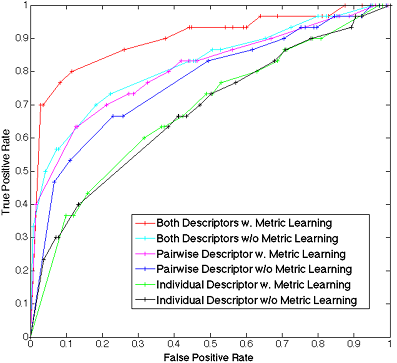
\includegraphics[width=2.4in]{ROC_s}
%\end{wrapfigure}

%We have evaluated this approach using a subset of the Harvard Interactive Classroom Dataset, to be described in Section~\ref{sec:sys}, which is orders of magnitude larger than existing interaction benchmarks~\cite{UTdata,Choi:context,Choi:recogtrack}), in terms of the number of individuals (10-50 students per camera), the number of cameras (6), and the amount of time (more than 50 camera-hours). Through a combination of face detection and tracking, we obtained noisy tracks for all students in each camera and computed simple descriptors based on absolute and pair-wise relative head pose. With input from educational experts we manually identified the participants and start/end times of 112 distinct three-person discussions, and we separated these into four semantically-meaningful categories (e.g., three sitting in a row with two facing left vs. two in front and one behind). The annotated interactions range from a few seconds to tens of seconds in length, and detecting and recognizing them is a challenge because the number of by-standers is much larger than the number of participants ($M$ is between 10 and 20 while $N=3$), video quality is limited (low light, less than 15fps), and the visual cues for interaction are quite subtle. Detection results obtained using a leave-one-session-out evaluation scheme are shown in the ROC curves at right, with various parts of the system being isolated, leaving only individual $\mathbf{f}$ or pairwise $\mathbf{g}$ descriptors, and atomic distance matrices $\Sigma_{I}$, $\Sigma_{P}$ set to identity instead of being data-optimized as will be described in Section~\ref{sec:actlearn}. These results suggest that our preliminary system approach works well, and its performance and flexibility are further supported by tests showing that it provides state-of-the-art detection and recognition results on existing interaction datasets involving both humans~\cite{UTdata} and mice~\cite{CRIM13}, exceeding the accuracy in~\cite{UTdata} by 21\% and exceeding the accuracy in \cite{CRIM13} by 8\%.



We have evaluated this approach using a subset of the Harvard Interactive Classroom Dataset, to be described in Section~\ref{sec:sys}, which is orders of magnitude larger than existing interaction benchmarks~\cite{UTdata,Choi:context,Choi:recogtrack}), in terms of the number of individuals (10-50 students per camera), the number of cameras (6), and the amount of time (more than 50 camera-hours). Through a combination of face detection and tracking, we obtained noisy tracks for all students in each camera and computed simple descriptors based on absolute and pair-wise relative head pose. With input from educational experts we annotated the participants and start/end times of 254 two-person and 112 three-person salient interactions separated into seven semantically-meaningful proxemes. The annotated interactions range from a few seconds to tens of seconds in length, and detecting and recognizing them is a challenge because the number of by-standers is much larger than the number of participants ($M$ is between 10 and 20 while $N=2,3$), video quality is limited (low light, less than 15fps), and the visual cues for interaction are subtle. Detailed results \cite{groupdet2013} suggest that our preliminary system works well on this data and also achieves state-of-the-art performances on benchmark datasets involving both humans~\cite{UTdata} and animals~\cite{CRIM13}.  
 
%While these early results are promising, they are only a small indication of what might be achieved. As part of the proposed activity, we will explore more sophisticated descriptor ensembles that allow, for example, larger cliques of relative descriptors and descriptors that are relative to the entire group. We will also explore measures of similarity that, instead of detection and recognition by matching, are well-suited for computing interaction saliency (i.e., interactions that are distinct from their space-time neighborhood) and for semi-supervised and unsupervised learning of categories (e.g., to automatically cluster the salient interactions discovered in a video collection).


While these early results are promising, they are only a small indication of what might be achieved. As part of the proposed activity, we will explore more sophisticated descriptor ensembles that allow, for example, \comment{larger cliques of} higher-order relative descriptors and descriptors that are relative to the entire group. We will explore explicit modeling of the temporal structures of the ensemble dynamics, resulting in an representation of "temporal parts" as a counterpart of the spatial parts model for static images \cite{pictorial1973,DPM2013}.We will also explore measures of similarity that, instead of by matching, are well-suited for computing proxeme distinctiveness (i.e., proxemes that are distinct from their space-time neighborhood). 


%We will also explore spatio-temporal search algorithms that preserve the robustness to false detections and broken tracks brought by voting but are more efficient in time.


%\subsubsection{Learning social interaction detectors and categories}
\subsubsection{Learning socially-informative proxeme categories}
\label{sec:actlearn}
\vspace{-5pt}

Given a set of pre-defined proxemes, we can detect and recognize instances of these categories using the methods of the previous section. However, to obtain these categories in another specific domain, another group of domain experts and extensive manual annotations are required, and in some domains there may not be experts or knowledge available \emph{a priori}. Meanwhile, commonly studied interactions categories \cite{UTdata} may not be informative: `kicking' and `punching'  are rare in reality, `hand-shaking' does not occur frequently between those with close relations, and `hugging' is too common to distinguish family relationship from professional peers.


\begin{wrapfigure}{r}{0.4\textwidth}
\vspace{-20pt}
  \begin{center}
    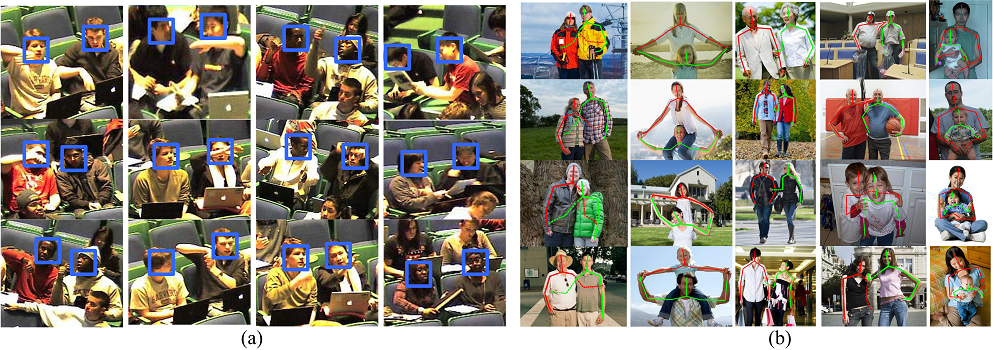
\includegraphics[width=0.4\textwidth]{socialdic}
  \end{center}
  \vspace{-20pt}
   \caption{ Socially-informative dictionary of proxemes of pairwise poses. Each column represents a proxeme.}
   \vspace{-15pt}
\label{fig:flicker}
\end{wrapfigure}
Therefore, our proposed activity includes to develop tools that allow unsupervised or semi-supervised learning of proxemes  that are informative for inferring social relationships, from observed interactions in various imagery collections such as online photo collections, TV show, and movies, as to be introduced in Section~\ref{sec:sys}. In contrast to a standard clustering problem, learning socially-informative proxemes requires to account for two major challenges. First, only a small subset of all observed interactions are useful proxemes, which necessitates the need for clustering ``selected" samples  in ``background clutter". Second, the algorithm must be able to effectively exploit side information, which might comes in the form of textual metadata or relationship information drawn from non-visual sources, once it is available. This side-information can be regarded as interaction signals from another ``domain'', and consequently might be exploited in borrowing from a domain adaptation framework recently developed by the PIs~\cite{LiZickler2012,Li2011}. 

In a preliminary experiment whose details are omitted due to space restriction, we unsupervisedly learned pair-wise pose proxemes from internet photos containing pair of individuals, where only locations of body key points were manually crowd-sourced. Figure~\ref{fig:flicker} shows five discovered proxemes (clusters), each shown in a column with four exemplars. We notice that even without side information, the discovered categories exhibit a statistically significant correlation with social relationships. The first column, where one person holds around the other's waist,  for example, shows a strong dominance of married couples or lovers. Our proposed research activity will include the development of a systematic scheme to discover richer and even more distinctive categories like these in larger scale, and establishing a dictionary of such visual proxemes as the bridge from imagery to social networks.





%Given a set of defined interaction categories, we can detect and recognize instances of these categories using the methods of the previous section. But how do we learn the categories in the first place? How can we make use of labeled samples of interactions? What if few labeled samples are present? In this subsection, we show preliminary results of using category-labeled interaction training samples to maximize the performance of detection and recognition described above, and we describe our plans for exploring semi-supervised and unsupervised learning.

%The detection and recognition system of Section~\ref{subsec:activity} incorporates learnable metrics $\Sigma_I$, $\Sigma_P$ for measuring ``atomic'' distances between descriptors in Eq.~\ref{eq:partial-matching}. These metrics can be optimized to improve detection by better discriminating between interactions and background, and when exemplars are labeled by category, they an be optimized to improve recognition by better discriminating between interaction categories. In our early experiments, we have shown that both of these can be accomplished simultaneously using an adaptation of the Large Margin Nearest Neighbor (LMNN) framework~\cite{Weinberger:ML}, and this is the procedure used to generate the ``w/ Metric Learning'' results in the previous section. It is one simple example of how annotations can be used to learn effective models for interaction categories, thereby allowing a single computational framework for interaction analysis to succeed in a wide variety of environments.

%We do this by constructing two collections from our database exemplars. The collection $\mathcal{P}$ contains all pairs of instantaneous interaction ensembles that are of the same category and occur roughly in the same temporal location within the interaction instances, together with their ``ground-truth" matchings. The collection $\mathcal{M}$, on the other hand, is comprised of ordered triples $(h,k,l)$ in which ensemble $h$ is the same category as ensemble $k$ and ensemble $l$ is either of a different category or background. Having defined these two collections, the Mahalanobis parameters are found by solving
%\begin{equation}
%\label{classify}
%\begin{split}
%&\min_{\Sigma_{I}, \Sigma_{P}} \sum_{(u,v)\in\mathcal{P}}\hat{D}(\mathcal{D}_{u}, \mathcal{D}_{v}, W_{u,v})+\gamma\sum_{(h,k,l)\in\mathcal{M}}\xi_{h,k,l},\\
%&\textup{s.t.}  \hat{D}(\mathcal{D}_{h}, \mathcal{D}_{l}, W)-\hat{D}(\mathcal{D}_{h}, \mathcal{D}_{k}, W_{h,k})\ge 2-\xi_{h,k,l}, \Sigma_{I}\succeq 0, \Sigma_{P}\succeq 0, \xi_{h,k,l}\ge0,
%\end{split}
%\end{equation}
%where $W_{u,v}$ is the ``ground-truth" matching for pair $(u,v)$ and $W$ is an arbitrary matching. The minimization over either $\Sigma_{I}$ or $\Sigma_{P}$ is exactly a Large Margin Nearest Neighbor (LMNN) problem \cite{Weinberger:ML}, and we apply LMNN multiple times to separately learn one distinct pair of ($\Sigma_{I}, \Sigma_{P}$) for each value of the number of interaction participants. 

%One of our goals in the proposed activity is to develop tools that allow effective learning of models for interaction categories with many fewer labeled samples. This is motivated by immense manual effort required to obtain these samples. We will explore semi-supervised and unsupervised methods for discovering interaction categories in video collections, based on measures of interaction saliency and between-ensemble similarity measures that incorporate loose space-time structural constraints. We will also explore the use of side information, which might comes in the form of textual metadata or relationship information drawn from non-visual sources. This side-information can be regarded as interaction signals from another ``domain'', and consequently might be exploited in a domain adaptation framework like those recently developed by the PIs~\cite{LiZickler2012,Li2011}. 


%%%%%%%%%%%%%%%%%%%%%%%%%%%%%%%%%%%%%%%%%%%%%%%%%%%%%%%%%%%%%%%%%%%%%%%%%%%%%%%%%%%%%%%%%%%%%%%


%\subsection{Salient Social Activities Discovery and Prediction}
%\label{sec:activity}
%
%The joint target recognition problem described in the previous section represent one scenario where social contexts significantly assist and improve a traditional computer vision task. In this section, we propose a \emph{new} computer vision task motivated and enabled by socialized metadata. This new task introduces new `words' that a picture or a video may convey, and the output conversely produces new clues for social sensing in related disciplines. 
%
%As the second major problem regarding socially-aware visual understanding, we propose to discover and predict salient social activities from videos, as well as still images if possible. The proposed task is novel from existing activity analysis and recognition work in three aspects: It seeks to discover salient social behaviors,  it  aims to predict activities using social contexts, and it directly builds upon realistic visual materials `in the wild'.
%
%\begin{figure}[t!]
%\begin{center}
%\includegraphics[width=\columnwidth]{socialbehavior}
%\end{center}
%\vspace{-0.25in} \caption{\captionsize 
%(a): Socially non-informative co-occurrence of articulations\cite{UTdata}; (b): Socially non-informative collective crowd activities\cite{Choi:context,Choi:recogtrack}; (c): Socially informative salient interactions; (d) Socially informative salient group interactions in the nature; (e) Socially meaningful three-way activity categories defined as `f-formations' by sociology\cite{Kendon1990}.\label{fig:socialbehavior}\afterfigspace}
%\end{figure}
%
%
%First, we propose to discover salient social activities. Specifically, social semantics assist in visual understanding in the way that they provide new social behavior categories for us to distill from images and videos, and these new social categories are informed by qualitative and quantitative sociology, which has been studying these behavior modes but never be automated by computer vision. As these new concepts are socially meaningful, they provide more expressive evidence about the social relationships among the individuals involved in the activities. We refer to these new social semantics as salient. In contrast to existing vision research, salient social activities are distinctive because they do not focus on non-informative interactions or group-wise behaviors. The non-informative interactions, for example, refer to the co-occurrences of two individual body articulations with limited clue about how the two individuals are related or exchange opinions, such as 'kick', 'punch', etc. (\cite{UTdata}, Fig. \ref{fig:socialbehavior}(a)). The non-informative group-wise behaviors, on the other hand, include collective activities of a crowd, within which there are no explicit interactions, such as 'group-walking', 'queueing', etc. (\cite{Choi:context,Choi:recogtrack}, \ref{fig:socialbehavior}(b)). Instead, the salient social activities are more  of gestural and conversational interactions, attention-response, as well as turn-taking meetings  (Fig \ref{fig:socialbehavior}(c)) where sociological semantics, as is interesting and important to the sociology research, can be derived. Fig. \ref{fig:socialbehavior} (e) shows diagrams for such socially meaningful activities categories, namely `f-formations', in three-way interactions that have been under the investigation of sociology. Moreover, we will develop generic salient socialized discovering models and approaches, so that they accommodate activities of social populations of animals and insects (Fig. \ref{fig:socialbehavior}(d)).
%
%Second, we propose to predict activities under social contexts. In this case, social semantics assist in visual understanding in the way that they serve as contextual information for restricting the more possible categories of activities that may occur between a specific group of individuals. This effort is also complementary to the usage of social contexts for identifying the targets presented in the previous section. Consider a simple illustrative example in which we would like to label a conversational scene in a movie as either a `negotiation� or a 'debate'. It is possible, in this case, that by the analysis of facial expressions, gestures, and poses, we still have difficulty in distinguishing the two. However, by appropriate face recognition in association with other metadata of the movie, probably with the help of social contexts as introduced in the previous section, we may gain solid confidence regarding the social relationship between the speakers as either `cooperative' or 'adverse'. A cooperative relationship are more likely to imply a negotiating activity, and an adverse relationship implies otherwise. A mechanism, similar to and in companion to the CRF formulation but adapted to video analysis, will be particularly useful.
%
%Third, we expect to develop approaches that directly take in realistic visual materials recording social activities of interest. On the one hand, realistic visual materials capture the social activities in unconstrained environment in the format of long-term surveillance videos of public areas with irrelevant human beings co-existing with socially engaged actors as well as scene/background clutter. Our approach will be one that can effectively and efficiently localize and retrieve salient social activities in space and time from these large volumes of cluttered image sequences. On the other hand, realistic visual materials such as surveillance videos and web videos are frequently in low and varying frame-rate, in low resolution, blurry, as well as in adverse view-points. Our effort will be handling all these realistic conditions and providing robust and practical tools that process more than those simulated, high-quality, manually pre-processed data \cite{UTdata,Choi:context,Choi:recogtrack}.
%
%\subsubsection{A prototype system and preliminary results}
%
%\begin{figure}[t!]
%\begin{center}
%\includegraphics[width=\columnwidth]{prototype}
%\end{center}
%\vspace{-0.25in} \caption{\captionsize 
%The prototype hardware and software infrastructure for analyzing socialized human behaviors in an indoor environment at Harvard University.\label{fig:prototype}\afterfigspace}
%\end{figure}
%
%As an initial attempt to analyze socialized human behaviors in an indoor environment, we have built up a prototype hardware and software infrastructure at Harvard University. As shown in Fig. \ref{fig:prototype}(a), the hardware part of the prototype system mainly consists of a networked audio-visual recording system for large-scale recording of student interactions in a Harvard College lecture hall. The system records audio and video from approximately one hundred students during each lecture in conjunction with the audience responses through an online teaching-learning application. The video system uses six IP cameras that together provide resolution that is high enough to achieve face-based identity recognition of each student in the audience. The audio system is an innovative design consisting 48 omnidirectional boundary microphones mounted inconspicuously among the seats, and outputting sound from each microphone recording to a single user-friendly mp3 audio file.To automatically analyze the videos, we have developed a robust computational suite of computer vision tools. This software consists of several fundamental modules that directly distill behavioral descriptions from raw videos, as well as a high-level module that detects salient social activities of interest from a new video and retrieves similar social activities. 
%
%
%With this established classroom observation system and these fundamental modules, we have successfully collected and processed a large-scale classroom behavior database consisting of 100 video clips in total. The students are seated in a regular lecture hall and are observed by a camera array with non-overlapping fields of view. The classroom is ``interactive'' because at various times throughout the lecture students are invited to engage in ad-hoc group discussions about problems provided by the instructor. The scale of our database is orders of magnitude larger than state-of-the-art computer vision datasets (e.g. those used in \cite{UTdata,Choi:context,Choi:recogtrack}), in the number of individuals (10-50 students per camera), the number of cameras (6), and the amount of time (100 minutes per camera, per recording, equaling over 3,000 minutes in total). Through a combination of face detection and tracking, we obtained noisy tracks for all students in each monocular video, upon which we developed descriptive modules that directly extract descriptiors such as head pose and body motion, we have also implemented a high-level module for behavior analysis based on similarity between two social groups, as depicted in Fig. \ref{fig:prototype}(b). In this module, the behavior of each individual is represented by a combination of the head pose and the motion of torso and arms (using the method of histogram of optical flows). The social behavior of a group is then represented by the configuration in space and time of the behaviors of its participants. With this social activity representation, the module detects a salient social activity from a new video and retrieves similar social activities from our established database. This functionality is illustrated in Fig. \ref{fig:prototype}(b), where our system has discovered a three-way conversation by identifying the participants of this conversation and the time span (several to tens of seconds) of this event. Based on the behavior representation for this space-time social interaction, the system searches the remainder of the database and retrieves a list of exemplars containing similar social behavior, ranked in the descending order of the similarities with the query. In this way, any manual annotations associated with the query video can be propagated to the top-ranking exemplars, and we are now taking this approach to propagate our manual annotations across the whole database. 
%
%
%\begin{figure}[t!]
%\begin{center}
%\includegraphics[width=\columnwidth]{dataset_compare}
%\end{center}
%\vspace{-0.25in} \caption{\captionsize 
%(a-1)-(a-3): Examples of the three categories for two-person interactions; (b-1)-(b-4): Examples of the four categories for three-person interactions; (c) Preliminary performance comparisons of our social activity retrieval software.\label{fig:dataset_compare}\afterfigspace}
%\end{figure}
%
%
%To evaluate the effectiveness of the social behavior retrieval module, we manually identified the participants and start/end times of all two-person, three-person, and four-person interactions, obtaining 254 two-person and 112 three-person interactions in total to constitute the entire database. In consultation with education experts we define interaction categories based on the geometric configurations of the participants: three categories for 2-person interactions (same row; different rows with left agent in front; different rows with right agent in front) and four categories for 3-person interactions. Example images for each category can be found in Fig. \ref{fig:dataset_compare}(a)(b). The annotated interactions range from a few seconds to tens of seconds in length. Since the raw videos arise from five different hour-long session, and we adopt a leave-one-session-out evaluation scheme in partitioning training samples (exemplars) from test samples (inputs). We study classification performance for 2-person and 3-person interactions, where we measure the accuracy of inferred interaction categories. Our low-level modules include both pose descriptors and relative motion descriptors, and our high-level module employs Metric Learning (ML). To evaluate the effectiveness of all these functionalities, we turned off some of components as baselines and compared with the full module with all components on. Fig. \ref{fig:dataset_compare}(c) shows the average true positive rates vs. false positives when classifying detected interactions into the three or four categories. As expected we see that performance improves when more parts of the system turned on, which implies that our prototype infrastructure has achieved reasonable technical quality.
%
%In our proposed research, we aim to enrich the descriptions of the social behaviors in the current prototype system, explore more accurate and robust comparison and retrieval mechanisms, and in particular, design novel modules for integrating social contextual annotations to allow our framework to be fully `socially-aware'.